% =============================================================================
% 片段 s02b：2.3 正则量子化、2.4 拓扑学的锦上添花
% 覆盖原文 p.9–13；编号公式 (2.20)–(2.31)；图 2（p.10）；脚注 3（p.11）
% 段落与原文一致：行内展示公式前后不留空行（原文为续段），仅在原文自然分段处空行
% =============================================================================

% ==== 原文 p.9 ====

\subsection{正则量子化}\label{sec:2.3}
% 原文标题：Canonical Quantization

% 原文标题：Classical treatment.
\paragraph{经典处理}现在转向哈密顿形式，看看它对 CS 理论的相空间能说些什么。先把 CS 作用量 \eqref{eq:2.1} 拆成 $A_0$ 与 $A_i$ 两部分，再分部积分：
\begin{equation}\tag{2.20}\label{eq:2.20}
  \SCS
  = \frac{k}{4\pi}\int_M \dd^3x\left(\varepsilon^{ij}A_i\dot A_j + 2A_0\varepsilon^{ij}\partial_iA_j\right)
  = \frac{k}{2\pi}\int_M \dd^3x\left(\frac12\varepsilon^{ij}A_i\dot A_j + A_0B\right).
\end{equation}
场 $A_0$ 在 $\SCS$ 中线性出现，且不带任何导数。它是循环坐标，通常称为非动力学场或拉格朗日乘子场。其运动方程为
\begin{equation}\tag{2.21}\label{eq:2.21}
  \frac{\partial \SCS}{\partial A_0} = 0
  \quad\Longrightarrow\quad
  \frac{k}{2\pi}B = \frac{k}{2\pi}F_{12} = 0.
\end{equation}
条件 $F_{12}=0$ 就是高斯定律约束；它排除磁单极子。

% [Tutor Note: 易错点] (2.20) 的 ε 分解：ε^{i0j}=−ε^{0ij} 令动能项反号，不能从 (2.1) 逐项复算
\begin{yizhu}[易错点]
把 \eqref{eq:2.1} 展开为 $\varepsilon^{0ij}A_0\partial_iA_j+\varepsilon^{i0j}A_i\partial_0A_j+\varepsilon^{ij0}A_i\partial_jA_0$。由 $\varepsilon^{i0j}=-\varepsilon^{0ij}$、$\varepsilon^{ij0}=+\varepsilon^{0ij}$，第三项分部积分后与第一项合并，给出 $2A_0B$；第二项却贡献 $-\varepsilon^{ij}A_i\dot A_j$，与 \eqref{eq:2.20} 所写的正号相反。而 $\varepsilon^{012}=+1$ 已由 \eqref{eq:2.4}、\eqref{eq:2.6} 的 $\rho=\frac{k}{2\pi}B$ 固定，故第一式并非 \eqref{eq:2.1} 的逐项展开。作者此后以 \eqref{eq:2.22} 的 $L$ 为准定出 \eqref{eq:2.23}，核对时不要单独翻转这一项。
\end{yizhu}

若在作用量层面施加此约束，就能丢掉 \eqref{eq:2.20} 的第二项：
\begin{equation}\tag{2.22}\label{eq:2.22}
  \SCS = \frac{k}{4\pi}\int_M \dd^3x\,\varepsilon^{ij}A_i\dot A_j .
\end{equation}
拉格朗日量 $\varepsilon^{ij}A_i\dot A_j$ 取正则形式 $L = p_i\dot x^i - H$：坐标 $x^i \propto \varepsilon^{ij}A_j$，动量 $p_i \propto A_i$，而（恒为零！）哈密顿量 $H = 0$。于是 $A_\mu = (0,A_1,A_2)$ 同时含动力学场与其共轭动量：它描述的是哈密顿量恒为零的理论相空间中的一点。遗憾的是，这些自由度是冗余的，因为 $A_\mu$ 在规范变换下非平凡地变换。

% ==== 原文 p.10 ====（本页首句是上一句的后半）

% 原文标题：Topological aside: CS on the torus.
\paragraph{拓扑插曲：环面上的 CS}事实上，理论中拓扑非平凡的威尔逊圈给出了 CS 相空间的一个规范不变参数化。$\R^3$ 与 $S^3$ 都单连通，其上纯 CS 理论中没有这类威尔逊圈。所以那里的 CS 相空间其实是空的！相比之下，我们在 \S\ref{sec:2.2} 中用源项手动引入了威尔逊圈。（另一种说法是：源的无穷大电荷密度引入了缺陷，改变了整体拓扑。）无论如何，我们对源的分析都等价于研究一个具有两个非平凡圈同伦类的流形上的纯 CS 理论；例如环面 $M = T^2\times\R$，其 $\pi_1(M) = \pi_1(T^2) = \Z\oplus\Z$。如图 \ref{fig:torus} 所示，这两个生成元给出上面讨论的两个威尔逊圈。两个 $W_i$ 都是取 $\mathrm{U}(1))$ 值的纯相位，所以环面上 CS 理论的经典相空间就是环面本身：$\mathcal{P} = \mathrm{U}(1))\times \mathrm{U}(1)) = T^2$。

\begin{figure}[htbp]
  \centering
  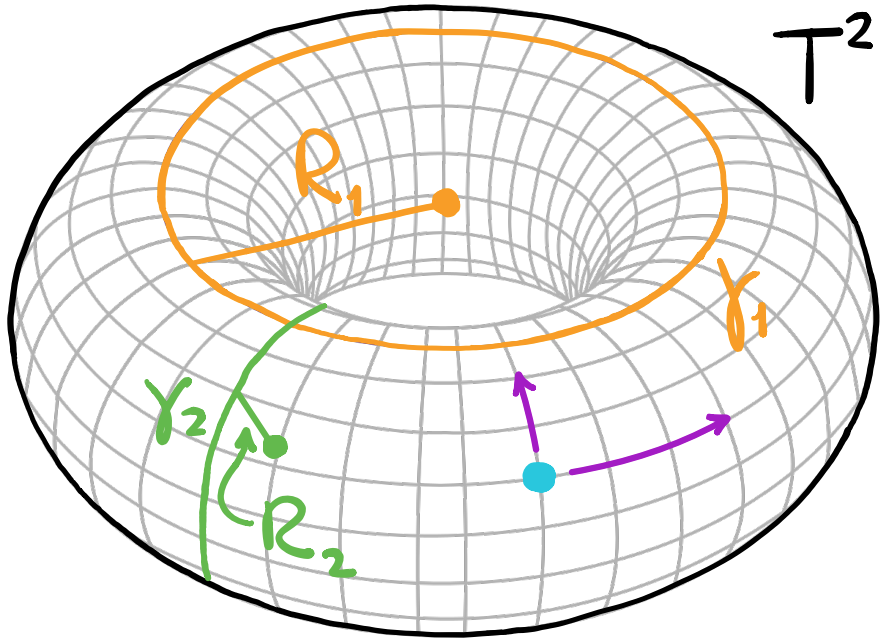
\includegraphics[width=0.5\textwidth]{figures/fig2_anyon_torus.png}
  \caption{一个在环面上运动的任意子。（原文 Figure 2，原文 p.10）}
  \label{fig:torus}
\end{figure}

% 原文标题：Canonical quantization.
\paragraph{正则量子化}规范理论的正则量子化分三步：(1) 固定一个规范，以施加规范不变性；(2) 施加所有非动力学约束；(3) 把正则泊松括号提升为对易子。这三步的先后不影响所得的量子理论；但（依理论而定）选错次序会带来难以逾越的困难。在目前的情形，我们从作用量 \eqref{eq:2.20} 出发，取 $A_0 = 0$ 规范，得到 \eqref{eq:2.22}。这一步等同于在作用量中施加约束 $F_{12} = 0$；不过须记住：高斯定律要在整个相空间上实施。在此阶段，运动方程的解仍未受约束，即它们可以有 $F_{12} = \partial_1A_2 - \partial_2A_1 \neq 0$。

这里我们选择先量子化、后施加约束：这一策略可行，因为运动方程与约束都对 $A$ 线性。在 \S\ref{sec:4} 中，我们会在高斯定律非线性的情形下采取相反的策略。
% ==== 原文 p.11 ====
正则泊松括号可直接从 \eqref{eq:2.22} 读出，随后把 $A_i$ 提升为算符：
\begin{equation}\tag{2.23}\label{eq:2.23}
  \{A_i(\mathbf x), A_j(\mathbf y)\}
  = \frac{2\pi}{k}\varepsilon_{ij}\delta^{(2)}(\mathbf x-\mathbf y)
  \ \rightsquigarrow\
  [A_i(\mathbf x), A_j(\mathbf y)]
  = \left(\frac{2\pi i}{k}\right)\varepsilon_{ij}\delta^{(2)}(\mathbf x-\mathbf y).
\end{equation}

% [Tutor Note: 易错点] 泊松括号换对易子要乘 i；(2.23) 的 ε_{ij} 与 (2.20) 的 ε^{ij} 混用上下标，不改符号
\begin{yizhu}[易错点]
正则量子化的替换规则是 $[\,\cdot\,,\cdot\,] = i\{\,\cdot\,,\cdot\,\}$，所以 \eqref{eq:2.23} 左式的 $2\pi/k$ 变成右式的 $2\pi i/k$：$i$ 只出现在对易子一侧，$k$ 仍在分母。又，此式两处都写 $\varepsilon_{ij}$（下标），而 \eqref{eq:2.20}、\eqref{eq:2.22} 用 $\varepsilon^{ij}$ 配 $A_i$；2 维空间里 $\varepsilon^{12}=\varepsilon_{12}=+1$，数值不变。这是作者混用上下标的习惯，不能据此补负号。
\end{yizhu}

% 原文标题：Solving the theory.
\paragraph{求解理论}现在来定基态波泛函 $\Psi_0[A(x)]$。这在场论中几乎做不到；不过在 $A_0 = 0$ 规范下 CS 作用量是二次的——理论自由——所以我们预期基态为高斯型。出于凝聚态理论中朗道能级的启发\footnote{另一种说法是：$A_0 = 0$ 规范把物理约化到平面 $\R^2 = \C$ 上，那里复坐标随手可得。\S\ref{sec:4} 关于全纯量子化的讨论也将呼应并拓展这一想法。}（见 \cite{dunne}），我们采用复坐标：
\begin{equation}\tag{2.24}\label{eq:2.24}
  z = x_1 + i x_2, \qquad A = A(z) = \sqrt{\frac{k}{2\pi}}\,(A_1 + iA_2).
\end{equation}
我们为基态取如下拟设，希望把它显式定出来：
\begin{equation}\tag{2.25}\label{eq:2.25}
  \Psi_0[A,\bar A] = \Psi[A(z)]\exp\left(-\frac12\int |A|^2\right).
\end{equation}
现在必须把 $F_{12} = 0$ 作为希尔伯特空间上的泛函方程施加。为此，先把对易子 \eqref{eq:2.23} 用重标度后的场 $A$ 与 $\bar A$ 改写，得到 $[A(z),\bar A(w)] = \delta(z-w)$。于是我们有权把 $A$ 看作“$x$”、把 $i\bar A$ 看作“$p$”，仿照量子力学写下 $\bar A = -\delta/\delta A$。这样 $F_{12} = \partial_1A_2 - \partial_2A_1$ 成了一个微分算子，可按（反）全纯导数 $\partial_\pm = \partial_1\mp i\partial_2$ 重新组织：
\begin{equation}\tag{2.26}\label{eq:2.26}
  F_{12}\Psi_0[A,\bar A]
  = \left(\partial_-\,\frac{\delta}{\delta A} + \partial_+A\right)\Psi_0[A,\bar A] = 0
  \quad\Longrightarrow\quad
  \left(\partial_-\,\frac{\delta}{\delta A} + \partial_+A\right)\Psi[A(z)] = 0.
\end{equation}
因子 $e^{-\frac12\int|A|^2}$ 消去，所得关于 $\Psi[A(z)]$ 的方程有高斯解：
\begin{equation}\tag{2.27}\label{eq:2.27}
  \Psi[A] \sim \exp\left[-\frac12\int A\left(\frac{\partial_+}{\partial_-}\right)A\right]
  \quad\Longrightarrow\quad
  \Psi_0[A(z)] = \exp\left(-\frac12\int\left[A\left(\frac{\partial_+}{\partial_-}\right)A + |A|^2\right]\right).
\end{equation}

% [Tutor Note: 易错点] (2.24) 的归一化：由 √(k/2π) 与 (2.23) 算得 [A,Ā]=2δ，与下文 [A,Ā]=δ(z−w) 差因子 2
\begin{yizhu}[易错点]
取 \eqref{eq:2.24} 的 $A=\sqrt{k/2\pi}\,(A_1+iA_2)$，代 \eqref{eq:2.23} 直接算得 $[A(z),\bar A(w)] = \frac{k}{2\pi}(-2i)\frac{2\pi i}{k}\delta^{(2)}(\mathbf x-\mathbf y) = 2\delta^{(2)}(\mathbf x-\mathbf y)$，而 \eqref{eq:2.26} 前原文写 $[A(z),\bar A(w)] = \delta(z-w)$。若约定 $\delta(z-w)=\delta^{(2)}(x-y)$，两式差因子 2；要让 $[A,\bar A]=\delta(z-w)$ 成立，\eqref{eq:2.24} 的 $2\pi$ 应换成 $4\pi$。作者随即用 $\bar A=-\delta/\delta A$，这套写法只与 $[A,\bar A]=\delta$ 配套；此处按原文的约定读，勿再乘 2。
\end{yizhu}

% [Tutor Note: 易错点] (2.26) 的 Ā=−δ/δA：符号由 [A,Ā]=δ 定死；∂± 定义不带 1/2
\begin{yizhu}[易错点]
$\bar A$ 在 \eqref{eq:2.26} 里实现为 $-\delta/\delta A$，地位等同量子力学中的 $p=-i\partial_x$：由 $[\delta/\delta A, A] = 1$ 得 $[A,-\delta/\delta A] = +\delta$；若漏掉负号，算符 \eqref{eq:2.26} 与高斯解 \eqref{eq:2.27} 会同时反号。另注意原文定义 $\partial_\pm = \partial_1\mp i\partial_2$ 不带 $\frac12$，与标准的 $\partial_z=\frac12(\partial_1-i\partial_2)$ 差因子 2；\eqref{eq:2.27} 中 $\partial_+/\partial_-$ 按原定义读，并记住它是形式算符之比。
\end{yizhu}

% [Tutor Note: 含糊点] 作者说 e^{−½∫|A|²} “drops out”，但 (2.27) 方括号里仍留 |A|²：它是被配方吸收的
\begin{yizhu}[含糊点]
作者称因子 $e^{-\frac12\int|A|^2}$ “drops out”，但 \eqref{eq:2.27} 的方括号里仍留着 $+|A|^2$：它并未消失，而是与高斯型解合并（配方）了。要从 \eqref{eq:2.26} 走到 \eqref{eq:2.27}，须把 $\bar A$ 实现为 $-\delta/\delta A$、把 $\partial_+/\partial_-$ 当成形式算符比，并处理二次型核的对称化；作者省略了这步代数。可对照 \cite{dunne} 的朗道能级波函数与 \cite{woodhouse} 的全纯量子化处理。
\end{yizhu}

% 原文标题：The torus again.
\paragraph{又见环面}前面我们研究过纯 CS 理论在环面上的经典相空间。现在手头有了对易子 \eqref{eq:2.23}，就可以量子化威尔逊圈了。我们写下 $W_a = e^{iw_a}$，其中 $w_a = \oint_{\gamma_a}\dd x^\mu_a A_\mu$。取 $A_0 = 0$ 规范，代入正则对易子 \eqref{eq:2.23} 并积分，得到 $[w_1,w_2] = \frac{2\pi i}{k}$。BCH 公式给出 $W_1$ 与 $W_2$ 所服从的代数：$W_1W_2 = e^{2\pi i/k}W_2W_1$。这一代数最小的非平凡表示维数为 $k\in\Z$，所以处在该表示中的场给出 $k$ 重基态简并。在亏格 $g$ 的曲面上，威尔逊圈更多；相应的代数也更复杂，基态简并度增长为 $k^g$。这种简并是新型拓扑物相的一个标志。

% [Tutor Note: 易错点] [w₁,w₂]=2πi/k 与 W₁W₂=e^{2πi/k}W₂W₁ 须配套：BCH 给出 e^{−2πi/k}，差号源于圈定向
\begin{yizhu}[易错点]
由 \eqref{eq:2.23} 沿两条生成圈积分得 $[w_1,w_2]=2\pi i/k$。再用 BCH：$e^{iw_1}e^{iw_2}=e^{i(w_1+w_2)}e^{-\frac12[w_1,w_2]}$，于是 $W_1W_2=e^{-2\pi i/k}W_2W_1$，与原文的 $e^{+2\pi i/k}$ 差一个符号。差异出在两条生成圈 $\gamma_1,\gamma_2$ 的定向（交点符号为 $\pm1$）；原文没有指定定向，故两式只能成套使用，不能各取一半。
\end{yizhu}

% [Tutor Note: 含糊点] “最小非平凡表示维数为 k”的理由：取 W₁^k W₂ 的迹得 ω^k=1，clock–shift 表示维数 k
\begin{yizhu}[含糊点]
作者直接断言“最小非平凡表示的维数为 $k\in\Z$”。理由：记 $\omega = e^{2\pi i/k}$，由 $W_1W_2 = \omega W_2W_1$ 得 $W_1^kW_2 = \omega^kW_2W_1^k$，两边取迹即要求 $\omega^k = 1$，故有限维表示只在 $k$ 为整数时存在；其不可约表示由时钟矩阵与移位矩阵给出，维数恰为 $k$，于是有 $k$ 重简并。亏格 $g$ 时每个把手贡献一对圈，简并度为 $k^g$。可参 \cite{witten1989} 与 \cite{verlinde1988}。
\end{yizhu}

% ==== 原文 p.12 ====

\subsection{拓扑学的锦上添花}\label{sec:2.4}
% 原文标题：Topological Bells and Whistles

% 原文标题：An invariant perspective.
\paragraph{不变量视角}看看无坐标的表述能为 CS 理论做点什么。先把 CS 作用量 \eqref{eq:2.1} 用微分形式重写：
\begin{equation}\tag{2.28}\label{eq:2.28}
  \SCS = \frac{k}{4\pi}\int_M A\wedge\dd A, \qquad A = A_\mu\dd x^\mu \in \Omega^1(M).
\end{equation}
CS 3-形式 $A\wedge\dd A$ 可定义在任何可定向 3-流形 $M$ 上，无需引用度规。它的积分是 $M$ 的拓扑不变量，尤其它在任意坐标变换下不变。如同在引力中那样，我们把坐标变换看作规范对称性。其中之一正是时间流动本身：相应的诺特荷——哈密顿量——必须恒等于零，这印证了 \S\ref{sec:2.3} 的正则分析。此外，$\SCS$ 不依赖度规，于是整个能动张量都为零：
\begin{equation}\tag{2.29}\label{eq:2.29}
  T^{\mu\nu}_{\mathrm{CS}} = \frac{2}{\sqrt{|g|}}\frac{\delta\mathcal{L}_{\mathrm{CS}}}{\delta g_{\mu\nu}} = 0.
\end{equation}
CS 理论与引力都具备这些特征——微分同胚不变性与 $H = 0$。事实上，3 维引力有一个一阶表述，就是一个 CS 理论 \cite{achucarro1986}！

% [Tutor Note: 物理图像] 作用量不含度规，便没有局部能动张量；H=0 即拓扑场论的定义性特征
\begin{yizhu}[物理图像]
作用量里没有度规，就无从对度规变分，能动张量只能为零：理论没有传播的局部自由度，能标出“物理”的只有拓扑。$H = 0$ 同理——时间平移本身是规范变换，所以没有能量，也就没有演化。这正是拓扑场论区别于普通场论的地方。
\end{yizhu}

% 原文标题：The θ term.
\paragraph{$\theta$ 项}微分形式的好处之一，是它澄清了 $\SCS$ 与 4 维杨–米尔斯理论中 $\theta$ 项的关系。主要想法 \cite{tong_gauge} 是把 $M$ 看成某个 4-流形 $X$ 的边界，再用斯托克斯定理与 $F = \dd A$ 写下
\begin{equation}\tag{2.30}\label{eq:2.30}
  S^{X}_{\mathrm{CS}}
  = \frac{k}{4\pi}\int_{\partial X} A\wedge\dd A
  = \frac{k}{4\pi}\int_X F\wedge F
  = \frac{k}{2\pi}\int_X \dd^4x\,F^{MN}\widetilde{F}_{MN} .
\end{equation}
这里我们在 $X$ 上给定一个度规，并用 $\widetilde{F}^{MN} = \frac12\varepsilon^{MNAB}F_{AB}$ 写出 $F\wedge F$ 的分量。（等价地，$F\wedge F$ 的积分就是 2-形式的霍奇内积 $\langle F,\star F\rangle$。）于是在整体归一化之内，CS 作用量就是一个 $\theta$ 项。

% [Tutor Note: 原文疑误] (2.30) 末项系数：k/4π∫F∧F = k/8π∫F^{MN}F̃_{MN}，原文写 k/2π，大 4 倍
\begin{yizhu}[原文疑误]
按 $F=\frac12F_{MN}\dd x^M\wedge\dd x^N$ 展开，$F\wedge F=\frac14\varepsilon^{MNAB}F_{MN}F_{AB}\dd^4x$；而 $\widetilde F^{MN}=\frac12\varepsilon^{MNAB}F_{AB}$ 给出 $F^{MN}\widetilde F_{MN}=\frac12\varepsilon^{MNAB}F_{MN}F_{AB}$，故 $\frac{k}{4\pi}\int F\wedge F=\frac{k}{8\pi}\int\dd^4x\,F^{MN}\widetilde F_{MN}$。\eqref{eq:2.30} 末一项写 $k/2\pi$，比正确系数大 4 倍。此处照录原文；\eqref{eq:2.31} 用的仍是 $k/4\pi$ 形式，故整性判据的结论不受影响。
\end{yizhu}

% 原文标题：Spin manifolds.
\paragraph{自旋流形}从 4 维视角看，$\SCS$ 只依赖 $F$，规范不变性是显然的。然而它现在关键地依赖我们对“体”时空 $X$ 的选择，而这不能成立。为使理论良定义，我们要求：任意两个有公共边界 $\partial X = \partial X' = M$ 的 4-流形 $X$、$X'$ 都满足 $S^{X}_{\mathrm{CS}} - S^{X'}_{\mathrm{CS}} \in 2\pi\Z$，以保持 \eqref{eq:2.12} 式的配分函数。重述这一判据的巧妙办法，是引入紧致 4-流形 $Y = (X\cup X')/M$：把 $X$ 与 $X'$ 沿公共边界 $M$ 以反转定向的方式粘起来。于是我们的要求读作
\begin{equation}\tag{2.31}\label{eq:2.31}
  S^{X}_{\mathrm{CS}} - S^{X'}_{\mathrm{CS}}
  = \frac{k}{4\pi}\int_Y F\wedge F \stackrel{!}{=} 2\pi n,
  \qquad n\in\Z.
\end{equation}
% ==== 原文 p.13 ====
结果表明，这一整性条件只在 $Y$ 是自旋流形时才成立；所谓自旋流形，就是能承载旋量的流形。例如 $T^4$、$S^4$ 与 $S^2\times S^2$ 都是自旋流形，而 $\mathbb{CP}^2$ 不是。至此，我们用几何解决了一个拓扑问题，并认识到：3 维 CS 理论与带费米子的 4 维规范理论有着内在联系。

% [Tutor Note: 含糊点] 整性只在自旋流形上成立：∫F∧F/4π² 为整数，自旋 4-流形相交形式为偶
\begin{yizhu}[含糊点]
作者称整性条件“只在 $Y$ 是自旋流形时成立”，未给证明。依据是：对 $\mathrm{U}(1))$ 丛，$\frac{1}{4\pi^2}\int_Y F\wedge F = \int c_1^2$ 为整数；自旋 4-流形的相交形式为偶（$w_2(Y)=0$ 的经典推论），故该整数为偶数 $2n$，于是 $\frac{k}{4\pi}\int F\wedge F = 2\pi kn$ 自动落在 $2\pi\Z$ 内。非自旋的 $\mathbb{CP}^2$ 相交形式为奇，只有偶数 $k$ 才相容。可参 \cite{witten1989} 与 \cite{aps1975}。
\end{yizhu}

% =============================================================================
% 汇报（供 Lead 汇总）
% 片段：2.3–2.4，原文 p.9–13
% 编号公式：(2.20)–(2.31) 共 12 个，均以 \tag 锁定；无编号展示公式：无
% 图 2 一处（fig:torus，p.10）；脚注 3 一处（p.11）
% 译注 10 条：易错点 5、含糊点 3、物理图像 1、原文疑误 1
% (2.30) 因子裁定：确认 SPEC §10 第 4 条成立。按 F=½F_{MN}dx^M∧dx^N 得
%   F∧F=¼ε^{MNAB}F_{MN}F_{AB}d^4x，而 F̃^{MN}=½ε^{MNAB}F_{AB}，故
%   (k/4π)∫F∧F=(k/8π)∫d^4x F^{MN}F̃_{MN}；原文末项写 k/2π，大 4 倍（4×k/8π）。
%   正文照录，已加「原文疑误」译注。(2.31) 仍用 k/4π 形式，结论不受影响。
% 其他核对结果：
%   1) (2.20)：由 (2.1) 按 ε^{012}=+1 展开，动能项应为 −ε^{ij}A_i\dot A_j，原文写 +；
%      与 (2.4)/(2.6) 定出的 ε^{0ij}=ε^{ij} 对照，仅动能项整体反号。作者以 (2.22)
%      的 L 定 (2.23)，故照录 + 批注（易错点）。SPEC §10 未列此条。
%   2) (2.24) 归一化：按 √(k/2π) 与 (2.23) 算得 [A,Ā]=2δ^{(2)}，原文下一段写
%      [A,Ā]=δ(z−w)，疑差因子 2（要自洽宜取 √(k/4π)）。照录 + 批注，存疑待裁定。
%   3) 环面：[w1,w2]=2πi/k 与 W1W2=e^{2πi/k}W2W1 依 BCH 差一符号，源自圈定向未定义；
%      照录 + 批注（SPEC §10 第 3 条的核对结论）。
%   4) p.11 提取文本 "correponding" 经图像核对为 "corresponding"，非笔误，不批注。
%   5) 跨片段引用：\eqref{eq:2.1}、\eqref{eq:2.4}、\eqref{eq:2.6}、\eqref{eq:2.12}、
%      \S\ref{sec:2.2}、\S\ref{sec:4}（需 s02a / s04a 的 label 与之一致）。
%   6) 段落：原文跨页处（p.9→p.10 尾句、p.10→p.11 "Poisson brackets"、p.12→p.13）
%      保持同段不断开，锚点注在段内相应位置。
% 自检：python tools/lint.py sections/s02b-abelian2.tex --tags 2.20,...,2.31 -> OK
% =============================================================================
